%----------------------------------------------------------------------------------------
%	PACKAGES AND OTHER DOCUMENT CONFIGURATIONS
%----------------------------------------------------------------------------------------

\documentclass[11pt]{article} % Default font size is 12pt, it can be changed here

\usepackage{graphicx} % Required for including pictures

\usepackage{float} % Allows putting an [H] in \begin{figure} to specify the exact location of the figure
\usepackage{wrapfig} % Allows in-line images such as the example fish picture
\usepackage[authoryear]{natbib}
\setcitestyle{square}
\bibliographystyle{agu08}
\usepackage{bibentry}
\usepackage[font=small,labelfont=sc]{caption}
\renewcommand\familydefault{\rmdefault}
\usepackage{charter}

\usepackage{titlesec}

\titleformat*{\section}{\normalsize\bfseries}
\titleformat*{\subsection}{\normalsize\bfseries}
% The following parameters seem to provide a reasonable page setup.
\topmargin 0.0cm
\oddsidemargin 0.2cm
\textwidth 16.5cm
\textheight 22cm
\footskip 1.0cm

\linespread{1.5} % Line spacing
\usepackage[usenames,dvipsnames,svgnames,table]{xcolor}
\usepackage[colorlinks]{hyperref}
\hypersetup{citecolor=Black}
\hypersetup{linkcolor=DarkRed}
\hypersetup{urlcolor=DarkBlue}
\usepackage{cleveref}

\let\OLDthebibliography\thebibliography
\renewcommand\thebibliography[1]{
  \OLDthebibliography{#1}
  \setlength{\parskip}{0pt}
  \setlength{\itemsep}{0pt plus 0.3ex}
}

%\setlength\parindent{0pt} % Uncomment to remove all indentation from paragraphs

\graphicspath{{figures/}} % Specifies the directory where pictures are stored

\begin{document}

%%%%%%%%%%%%%%%%%%%%%%%%%%%%%%%%%%%%%%%%%%%%%%%%%%%%%%%%%%%%%%%%%%%%%%%%%%%%%%%%
% PAPER BODY
%%%%%%%%%%%%%%%%%%%%%%%%%%%%%%%%%%%%%%%%%%%%%%%%%%%%%%%%%%%%%%%%%%%%%%%%%%%%%%%%

\section{Introduction}


\section{Methods}
\subsection{Observational Data}
Paragraph about the Line-W observational data.

Paragraph about the age calculation.

Regridding of observational data

\subsection{Model Simulation}
Because of limited observational temporal and spatial resolution, we additionally
use data from a pre-industrial control model simulation to investigate the
relationship between age and oxygen along Line-W.  We use the GFDL ESM2Mc
\citep{Galbraith2011}, a coarse resolution configuration of the GFDL ESM2M
\citep{Dunne2012}. For a more complete description of the model configuration and
simulation please reference the methods section in \textit{Thomas et al.,} 2017.

\section{Results}
\subsection{Observations}

Figure 1 shows the mean age and oxygen observations along Line-W for two years -
November 2003 and August 2012. These years were chosen for display purposes because
they have the best spatial data resolution. Comparing the oxygen concentration (left)
against the mean age (right), we see an overall (opposite) similarity in the
spatial pattern. I'm not sure what else to discuss about this figure.

In order to more directly compare the relationship between mean age and oxygen,
we calculated the correlation between the two variables (Figure 2 a). The
anticipated negative correlation is present through most of the domain with exception
of two positive correlation regions. One region at a depth of approximately 500 m
and a second, larger region spanning depths 1250 m -- 2000 m. It should be noted that
due to limited data availability, the finer details of the correlations in the
observational data should not be trusted. For that reason we will only consider
the large scale patterns of the correlation, and supplement this analysis with
model simulation analysis in the next section.

Because oxygen is dependent on both biological consumption and changes in temperature
(solubility), it can be difficult to interpret patterns in oxygen concentration or
in this case the age-oxygen correlation. To remove the impacts of solubility, we
also consider the Apparent Oxygen Utilization (AOU). AOU is the difference between
the oxygen saturation and the observed oxygen concentration. The correlation
between mean age and AOU is shown in Figure 2 b. In this case, the upper region of
(now negative) anomalous correlation goes away (or is much smaller), while the bottom
region of anomalous correlation remains. This suggests that the region at the 500 m
depth is primarily being influenced by changes in the oxygen saturation.

In order to better understand why these positive regions of correlation exist, we
show the scatter plot of mean age versus oxygen and AOU in Figure 3. The scatter plot
between age and oxygen (Figure 3 a) shows an S-shape that roughly follows depth.
The approximate depth levels are also shown. In an ideal world I would also color
the scatter plot to show that the areas of positive correlation occur as the `bends'
in the S-shape (as I do for the model data). Same with the age-AOU scatter plot.

And this is the end of my observational data analysis\ldots it's awesome I know.

Comparison of observational data to model data.

Analysis of model data to explain why positive correlation regions are there.


{\footnotesize
   \bibliography{/RESEARCH/library}
}

\clearpage

\begin{figure}
\noindent
\centering
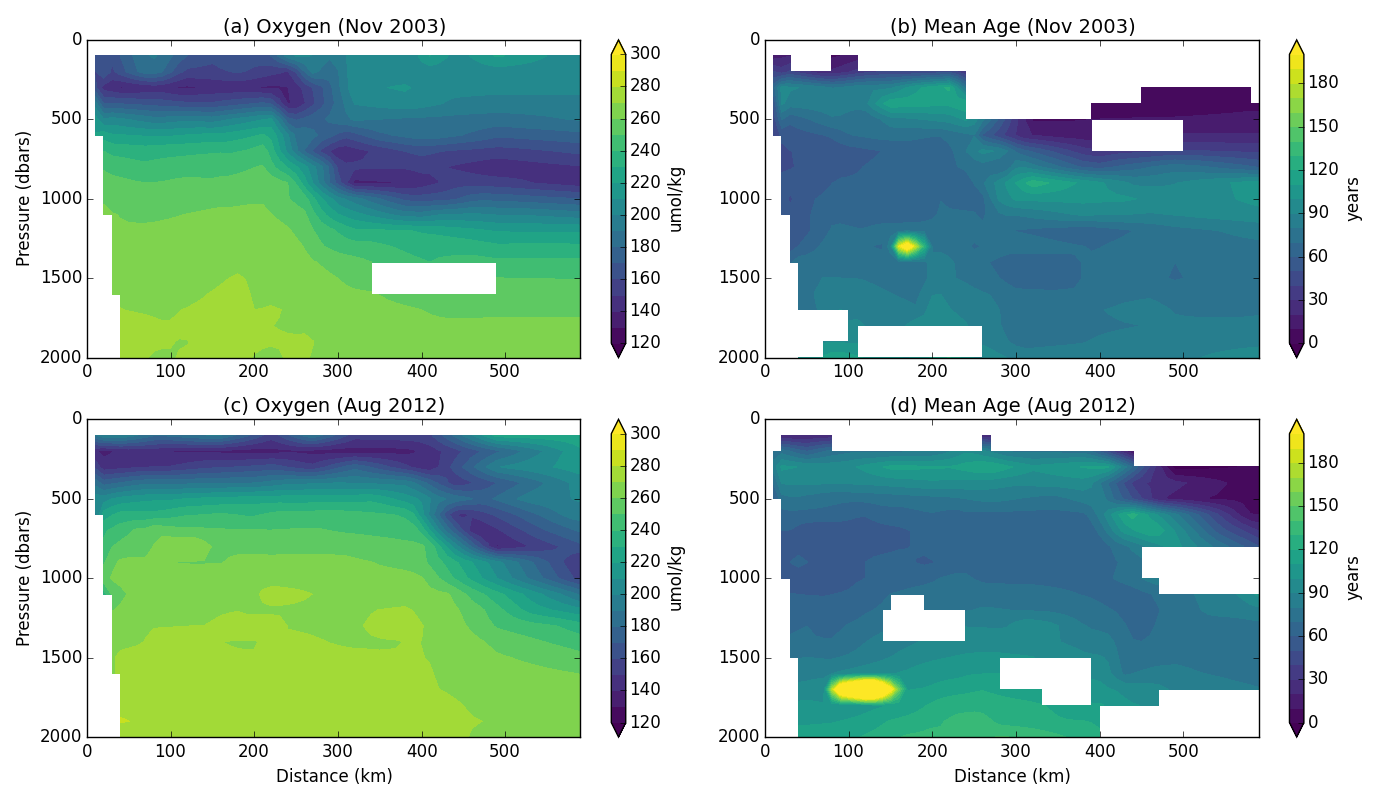
\includegraphics[width=43pc]{age_oxygen_figure1.png}
\caption{Observations along Line-W for (left) oxygen concentration and (right)
mean age for observation years (top) November 2003 and (bottom) August 2012.}
\label{fig:obs_age_o2_contour}
\end{figure}

\begin{figure}
\noindent
\centering
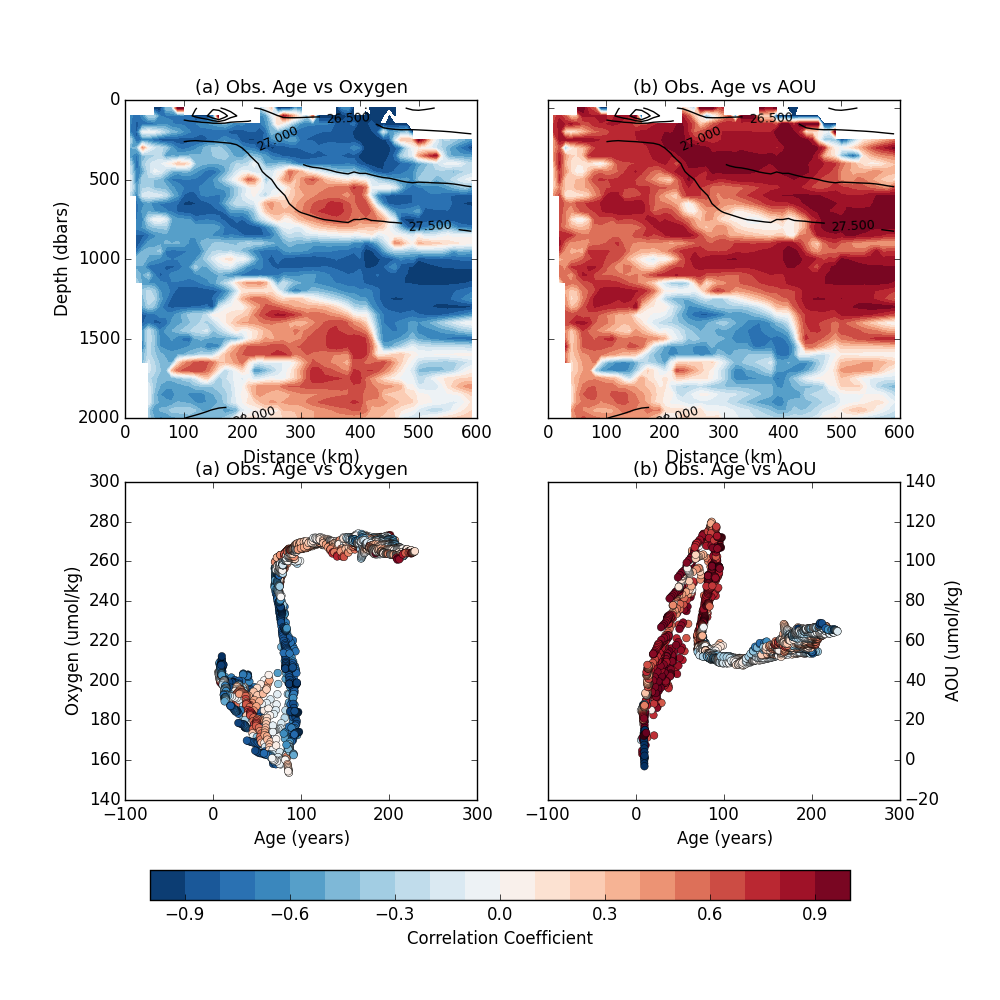
\includegraphics[width=43pc]{age_oxygen_correlation.png}
\caption{Pearson correlation coefficients for age versus (left) oxygen and (right)
AOU for both (top) Line W observations and (bottom) ESM2Mc model interpolated to
Line W. Contour lines indicate neutral density climatology.}
\label{fig:obs_age_o2_contour}
\end{figure}

\begin{figure}
\noindent
\centering
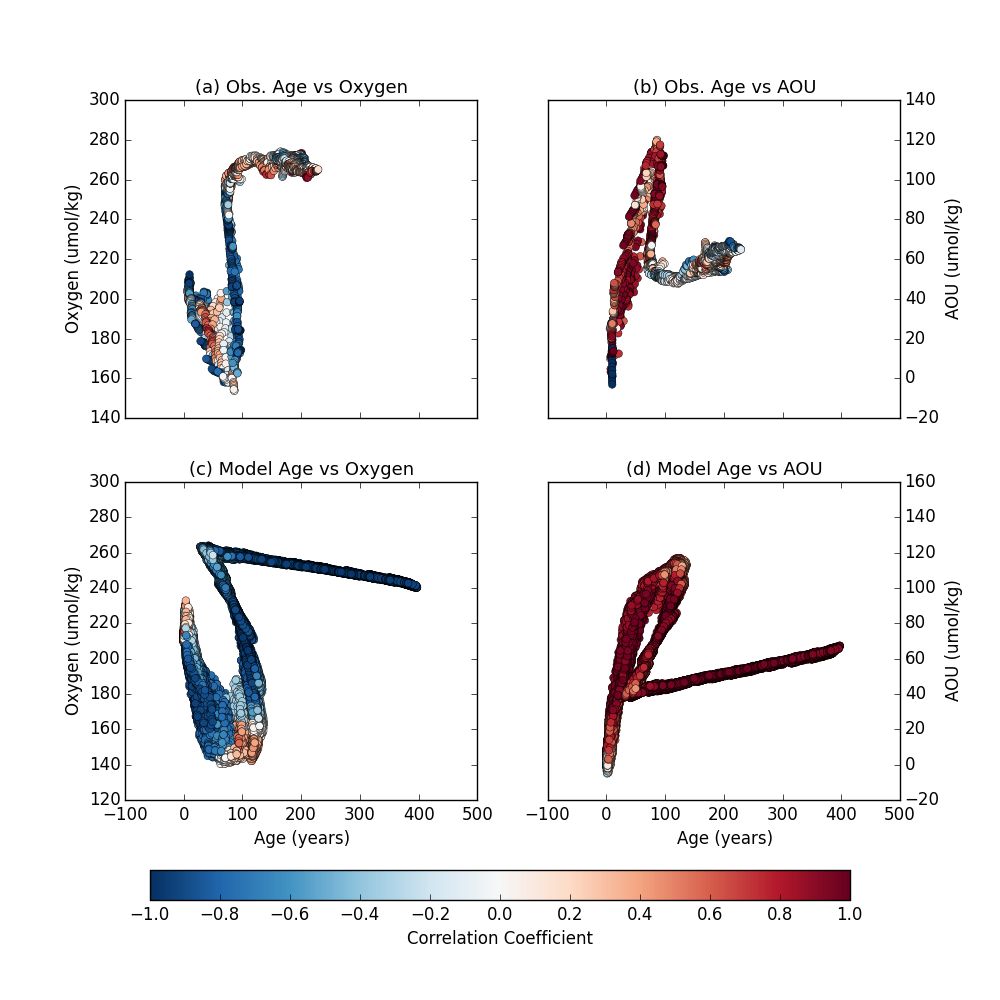
\includegraphics[width=43pc]{age_oxygen_scatter.png}
\caption{Scatter plots for age versus (left) oxygen and (right)
AOU for both (top) Line W observations and (bottom) ESM2Mc model interpolated to
Line W. Note scatter plot is colored to represent each points correlation coefficient between
the respective variables.}
\label{fig:obs_age_o2_contour}
\end{figure}


\begin{figure}
\noindent
\centering
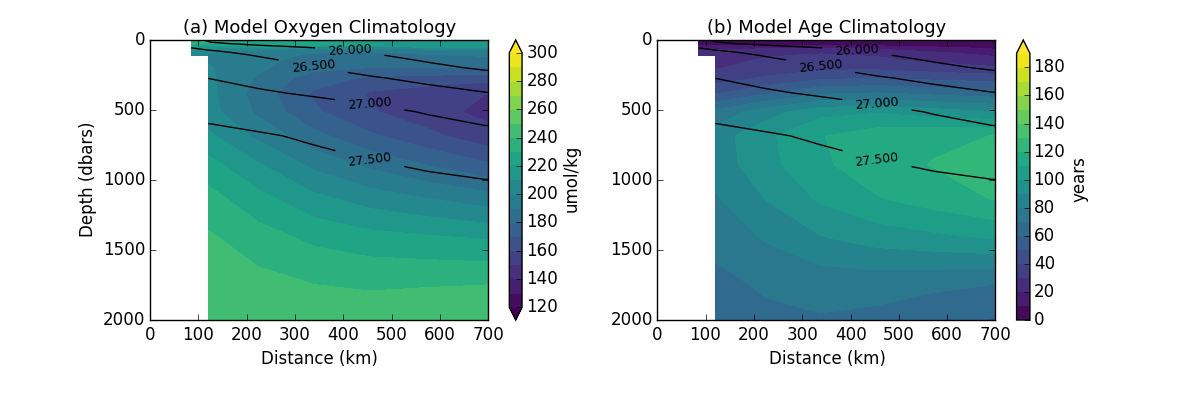
\includegraphics[width=45pc]{age_oxygen_model_clim.png}
\caption{Model climatology for (a) oxygen and (b) ideal age. Black contour lines
represent mean neutral density. }
\label{fig:obs_age_o2_contour}
\end{figure}


\end{document}
